\documentclass[twocolumn, 10pt,a4j]{jsarticle}
  \usepackage{amsmath}
  \usepackage{here}
  \usepackage[dvipdfmx]{graphicx}
  \usepackage{url}
  % プリアンブル
  \title{\vspace{-2.5cm}振動の計測と制御}
  \author{1610581 堀田 大地}
  \date{2018/7/26}
  \begin{document}
  \maketitle{}

  
  \begin{figure}[H]
    % 図1
    \begin{center}
      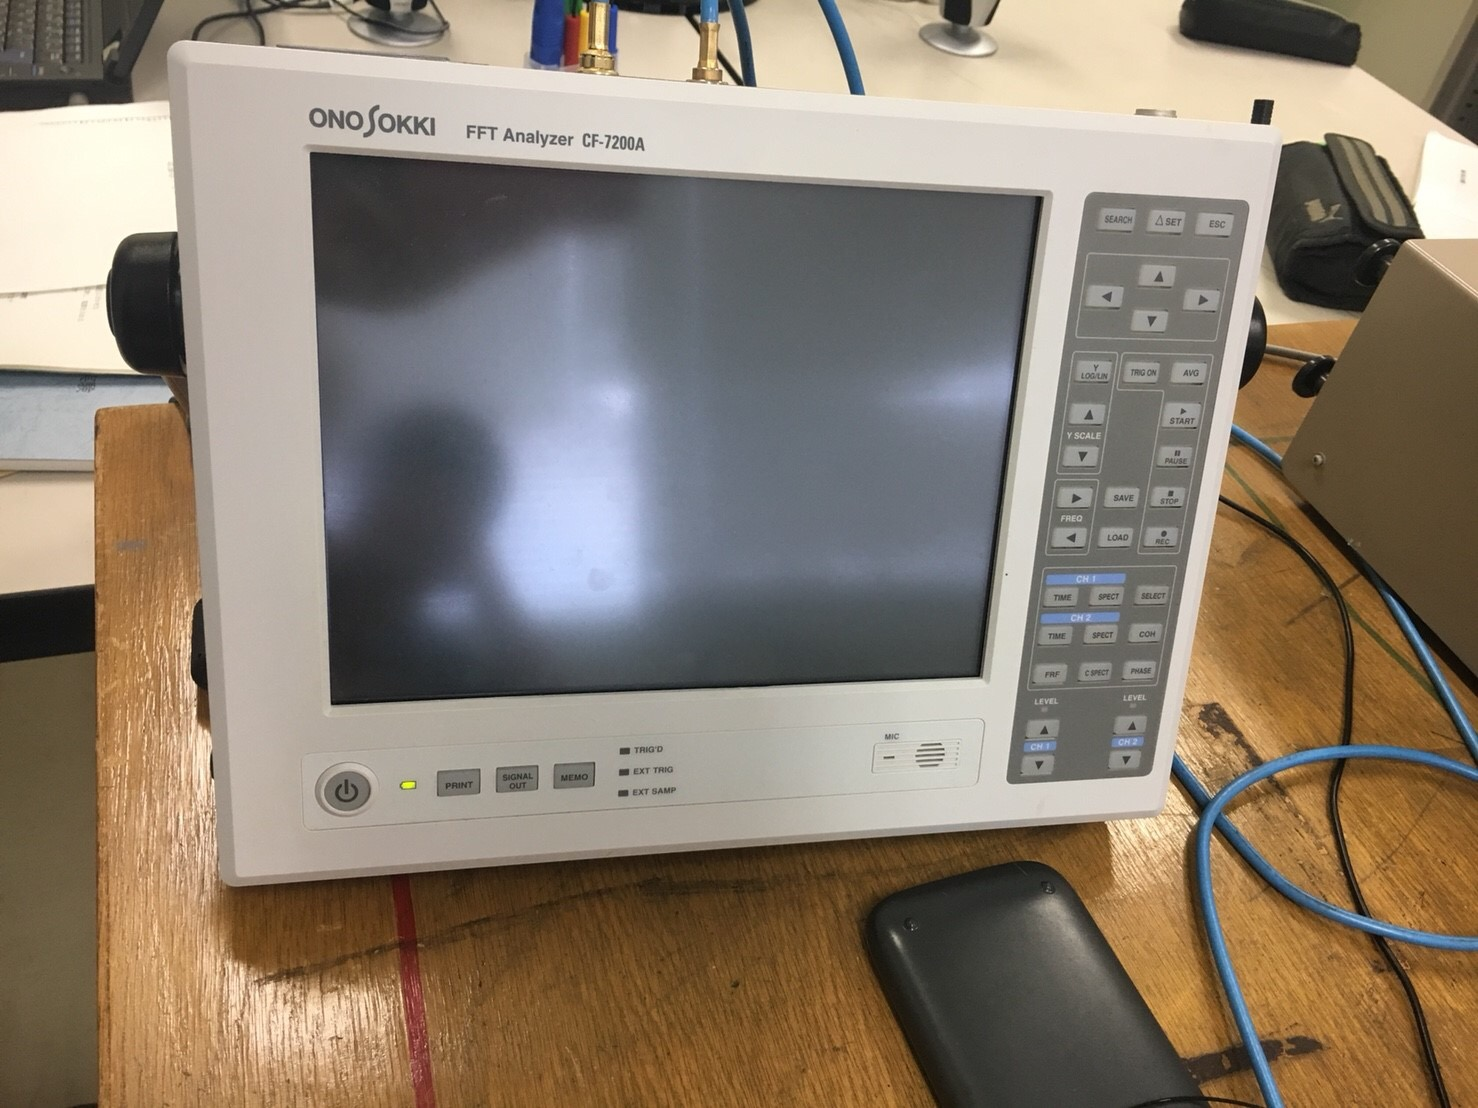
\includegraphics[width=7cm]{../img/IMG_3030.JPG}
      \caption{FFTアナライザ.入力電圧をフーリエ変換して周波数にして表示する端末.}
    \end{center}
  \end{figure}

  \begin{figure}[H]
    % 図2
    \begin{center}
      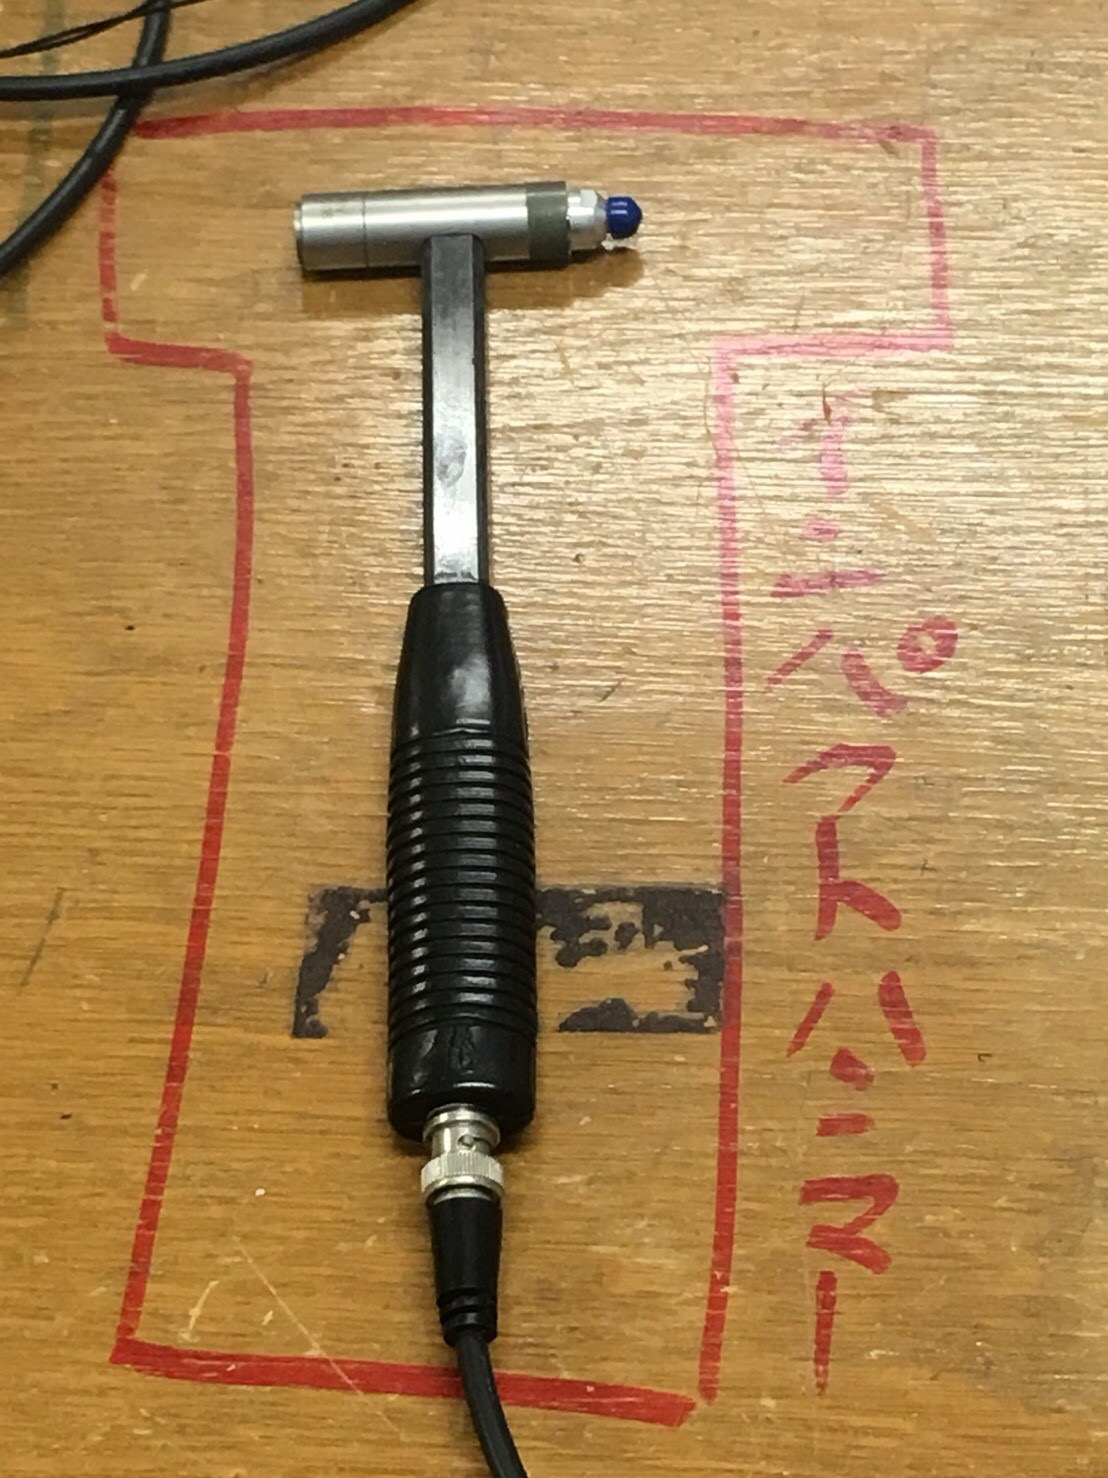
\includegraphics[width=7cm]{../img/IMG_3027.JPG}
      \caption{インパクトハンマー.衝撃を生じさせて振動を生み出すハンマ-.}
    \end{center}
  \end{figure}

  \begin{figure}[H]
    % 図3
    \begin{center}
      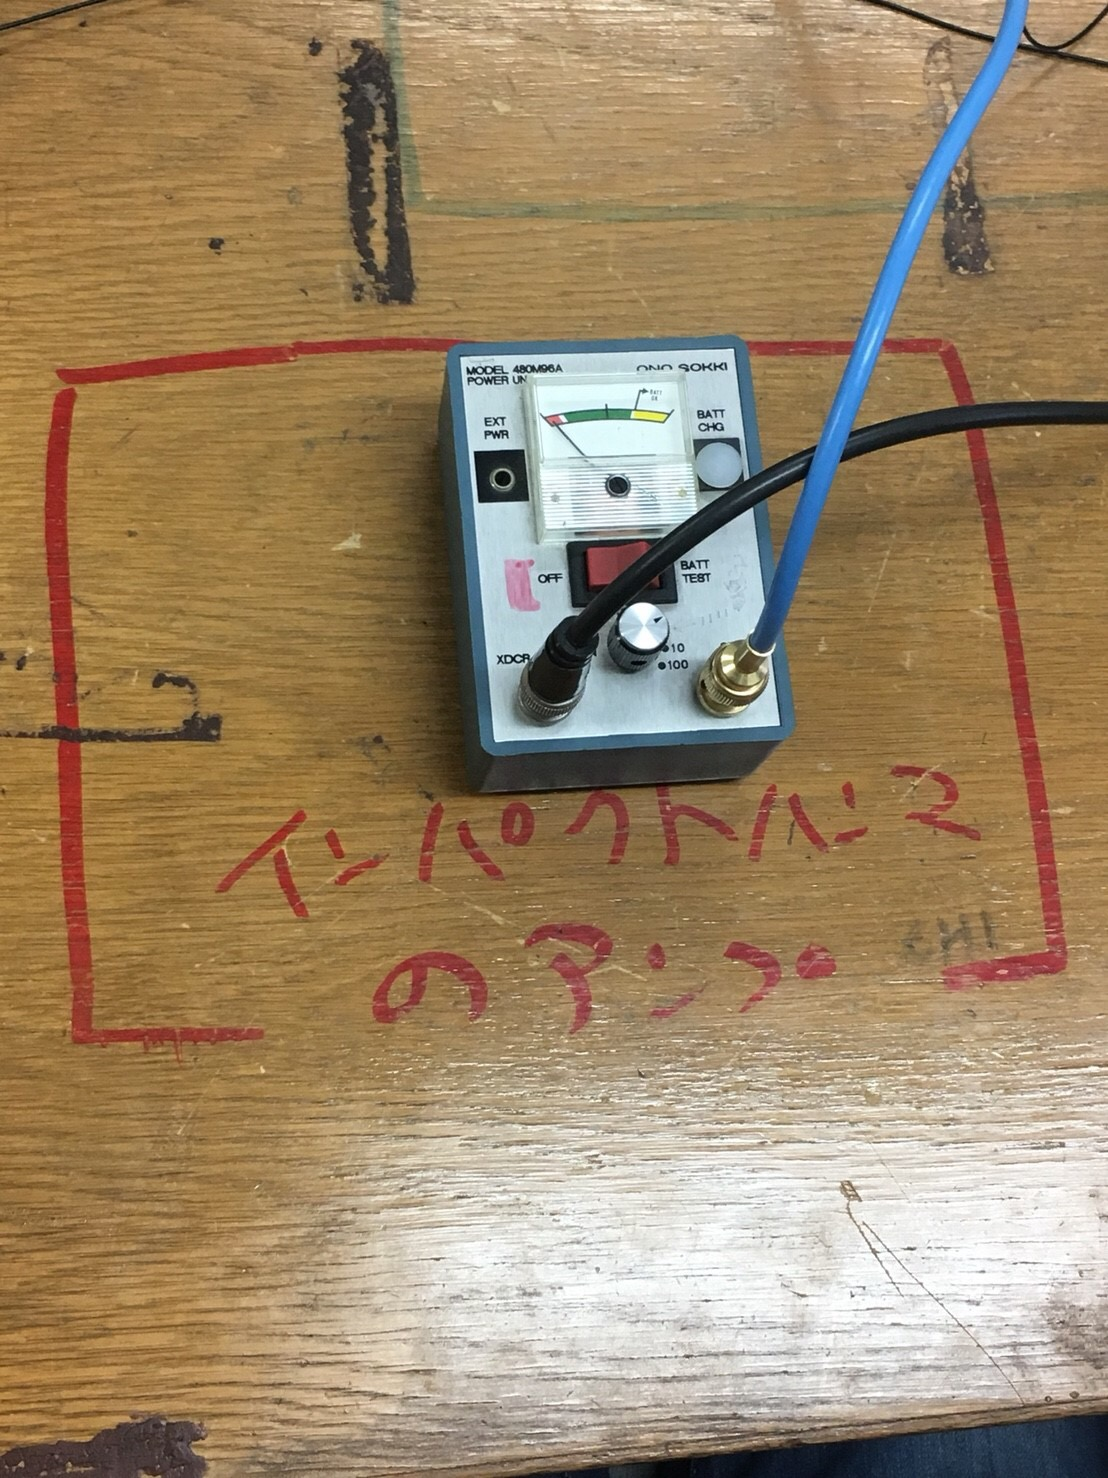
\includegraphics[width=7cm]{../img/IMG_3028.JPG}
      \caption{インパクトハンマーのアンプ.衝撃の振幅を増幅させる装置.}
    \end{center}
  \end{figure}

  \begin{figure}[H]
    % 図4
    \begin{center}
      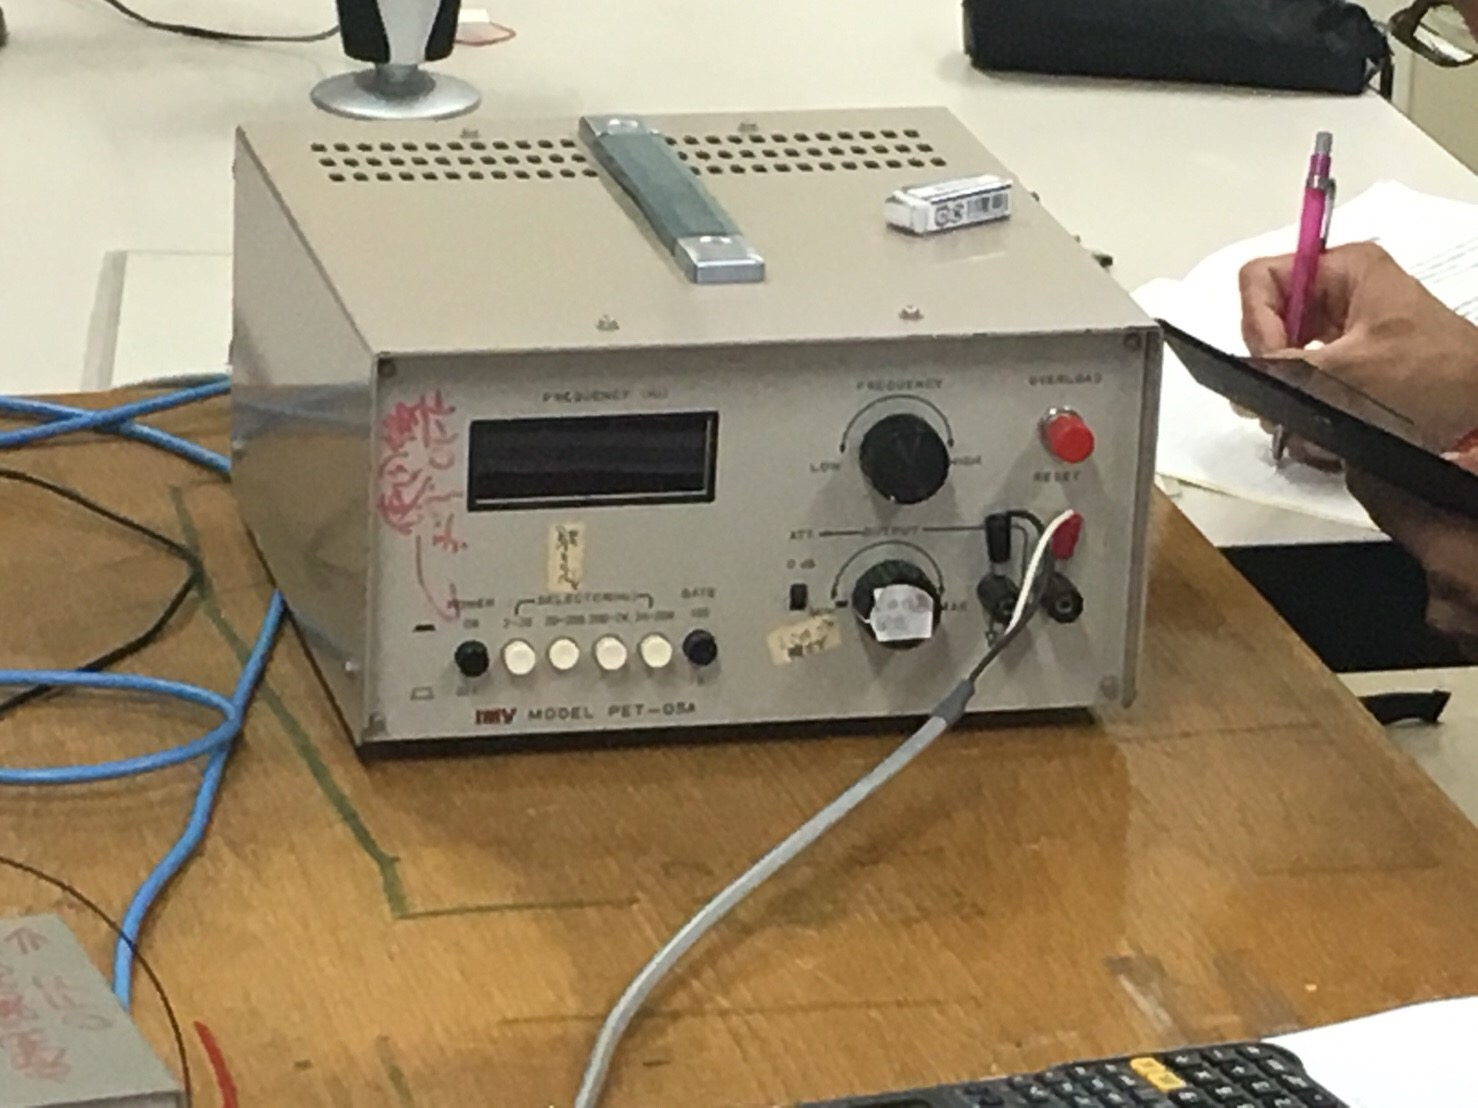
\includegraphics[width=7cm]{../img/IMG_3024.JPG}
      \caption{電圧を送る機械.}
    \end{center}
  \end{figure}

  \begin{figure}[H]
    % 図5
    \begin{center}
      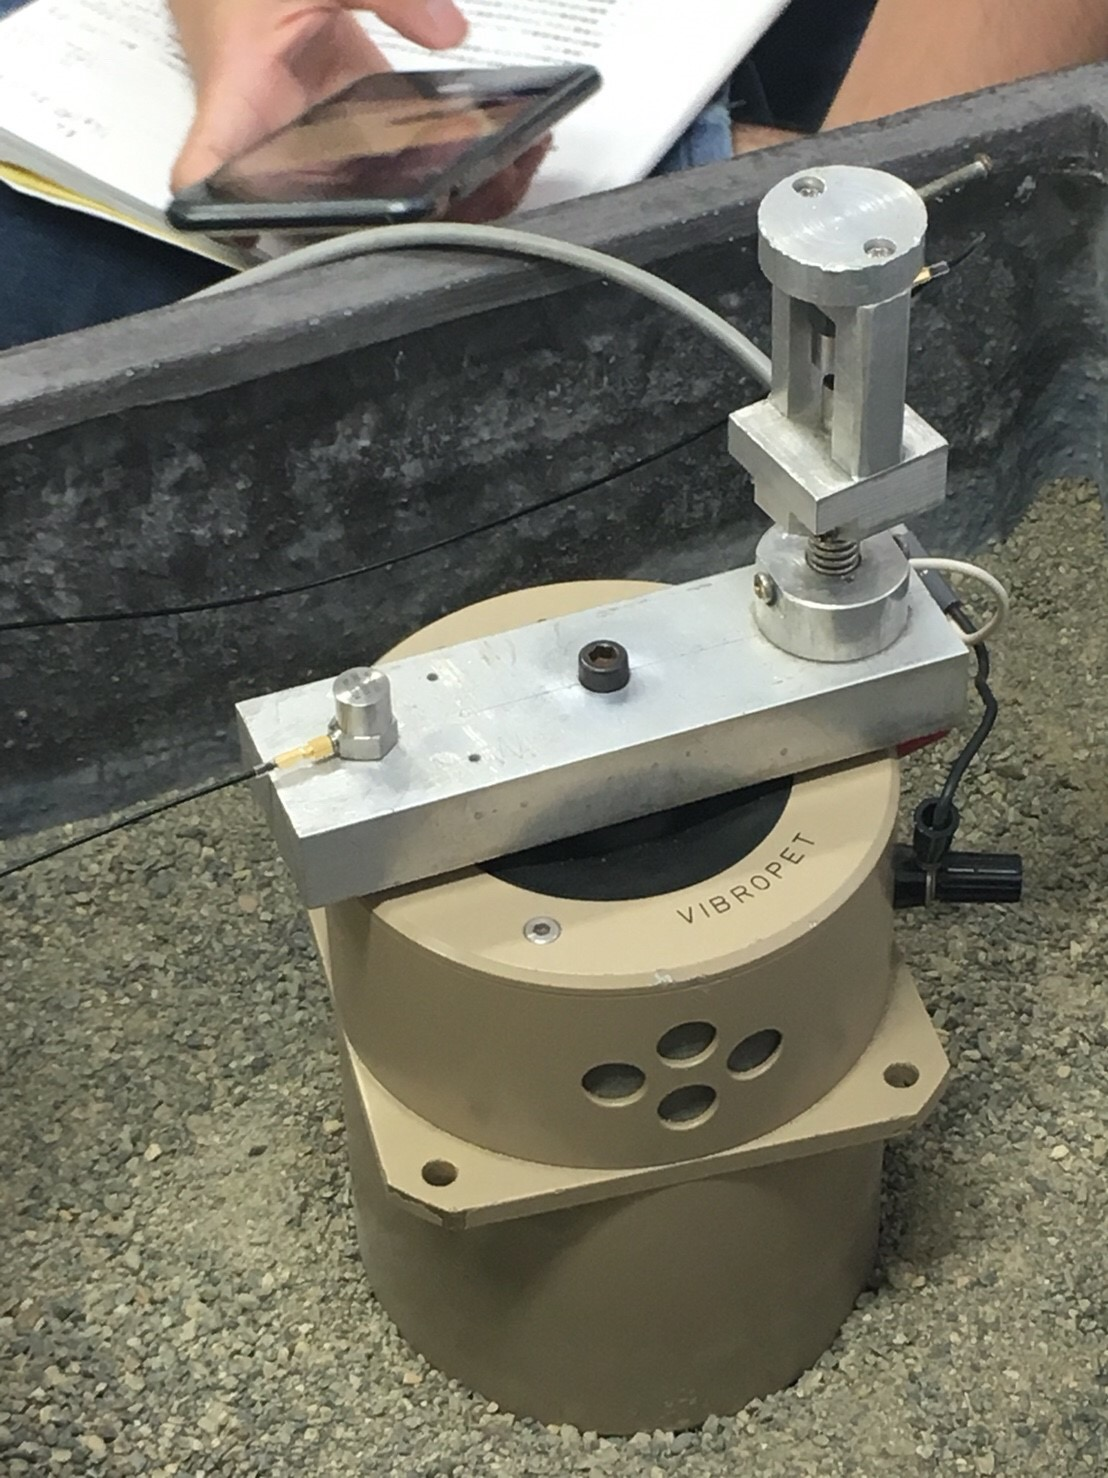
\includegraphics[width=7cm]{../img/IMG_3025.JPG}
      \caption{加速度センサーをつけたばね振動系.}
    \end{center}
  \end{figure}

  \begin{figure}[H]
    % 図6
    \begin{center}
      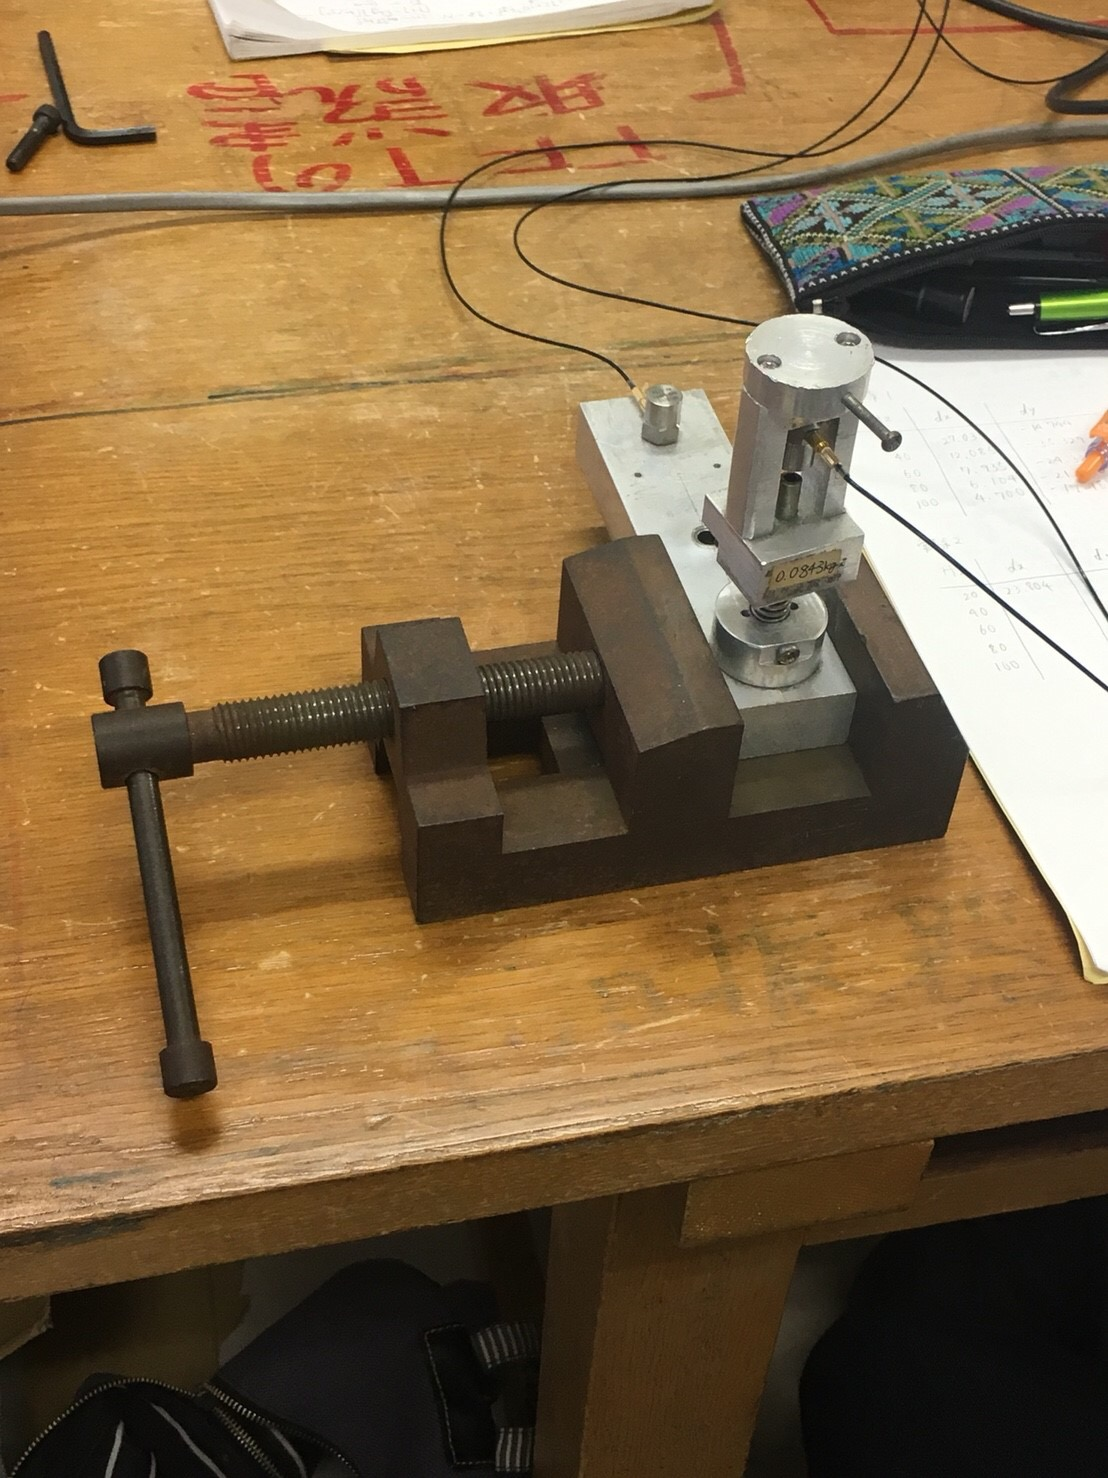
\includegraphics[width=7cm]{../img/IMG_3026.JPG}
      \caption{加振器.振動を送り物体を揺らす.}
    \end{center}
  \end{figure}

  \begin{figure}[H]
    % 図7
    \begin{center}
      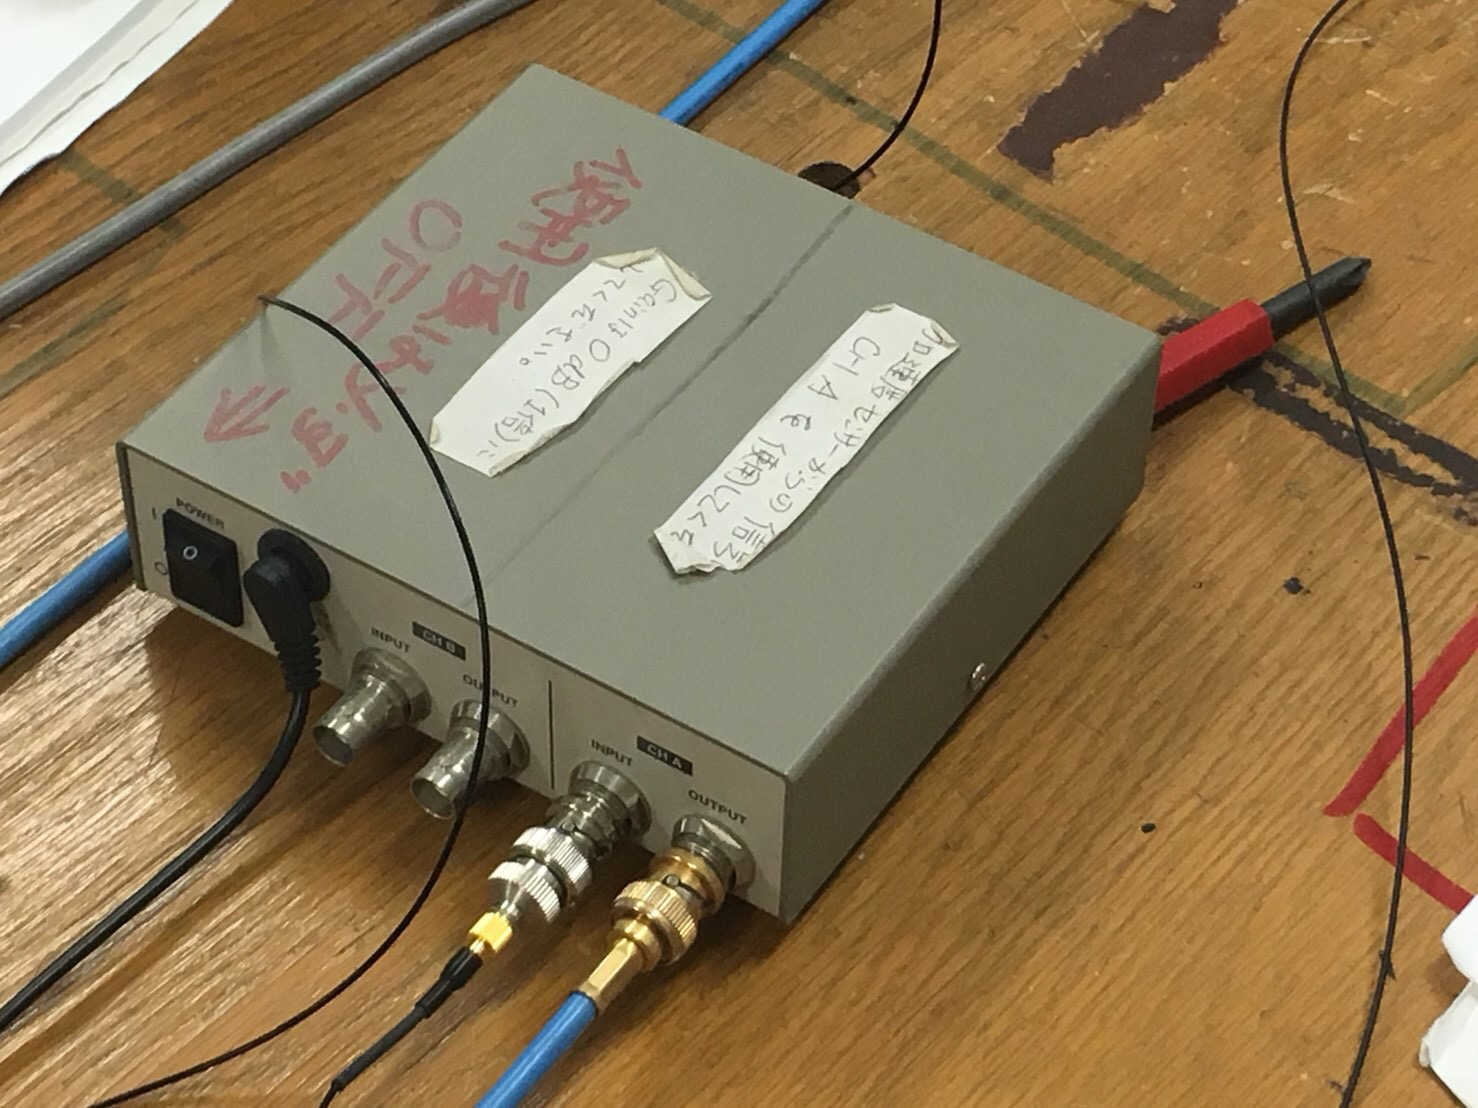
\includegraphics[width=7cm]{../img/IMG_3029.JPG}
      \caption{増幅器.波の振幅を増幅させる.}
    \end{center}
  \end{figure}

  \end{document}